% This LaTeX document needs to be compiled with XeLaTeX.
% !TeX program = xelatex
\documentclass[10pt]{article}
\usepackage[utf8]{inputenc}
\usepackage{ucharclasses}
\usepackage{amsmath}
\usepackage{amsfonts}
\usepackage{amssymb}
\usepackage[version=4]{mhchem}
\usepackage{stmaryrd}
\usepackage{bbold}
\usepackage{graphicx}
\usepackage[export]{adjustbox}
\graphicspath{ {./images/} }
\usepackage{caption}
\usepackage{fvextra, csquotes}
\usepackage{polyglossia}
\usepackage{fontspec}
\usepackage{newunicodechar}
\setmainlanguage{spanish}
\setotherlanguages{tamil}
\IfFontExistsTF{Noto Serif Tamil}
{\newfontfamily\tamilfont{Noto Serif Tamil}}
{\IfFontExistsTF{Tamil MN}
  {\newfontfamily\tamilfont{Tamil MN}}
  {\IfFontExistsTF{Lohit Tamil}
    {\newfontfamily\tamilfont{Lohit Tamil}}
    {\IfFontExistsTF{FreeSerif}
      {\newfontfamily\tamilfont{FreeSerif}}
      {\newfontfamily\tamilfont{Latha}}
}}}
\IfFontExistsTF{CMU Serif}
{\newfontfamily\lgcfont{CMU Serif}}
{\IfFontExistsTF{DejaVu Sans}
  {\newfontfamily\lgcfont{DejaVu Sans}}
  {\newfontfamily\lgcfont{Georgia}}
}
\setDefaultTransitions{\lgcfont}{}
\setTransitionsFor{Tamil}{\tamilfont}{\lgcfont}

\newunicodechar{→}{\ifmmode\rightarrow\else{$\rightarrow$}\fi}
\newunicodechar{∴}{\ifmmode\therefore\else{$\therefore$}\fi}
\newunicodechar{□}{\ifmmode\square\else{$\square$}\fi}
\newunicodechar{⋯}{\ifmmode\cdots\else{$\cdots$}\fi}

\begin{document}
\captionsetup{singlelinecheck=false}
\section*{Z}
\section*{Preuniversitario Zenit}
\section*{CAPÍTULO 1}
\section*{NÚMEROS ENTEROS}
"Ha sido un largo camino, pero aquí estoy"\\
Fotografié mapaches en una playa de Florida, donde les di de comer camarones. Luego este me dio las gracias así.

\begin{itemize}
  \item FOTÓGRAFÍA: JENNIFER HADLEY -
\end{itemize}

FUENTE: THE COMEDY WILDLIFE PHOTO

\section*{CAPÍTULO 1}
\section*{"Vive como si fueses a morir mañana. Aprende como si fueses a vivir siempre"}
\begin{itemize}
  \item MAHATMA GANDHI -
\end{itemize}

ABOGADO, PENSADOR Y POLÍTICO

\begin{enumerate}
  \item CONJUNTOS NUMÉRICOS\\
a. Números enteros\\
b. Valor absoluto
  \item ORDEN EN EL CONJUNTO DE LOS NÚMEROS ENTEROS
  \item LAS CUATRO OPERACIONES BÁSICAS EN LOS ENTEROS\\
a. Adición y Sustracción\\
b. Multiplicación y División
  \item MÚLTIPLOS Y DIVISORES\\
a. Múltiplos\\
b. Divisores
  \item PARIDAD E IMPARIDAD
  \item PROPIEDADES DE LAS OPERACIONES EN LOS NÚMEROS ENTEROS\\
a. Propiedad Conmutativa\\
b. Propiedad Asociativa\\
c. Propiedad Distributiva\\
d. Neutro Aditivo y Neutro Multiplicativo\\
e. Inverso Aditivo\\
f. Elemento Absorbente\\
g. Prioridad de las operaciones
  \item CRITERIOS DE DIVISIBILIDAD
  \item NÚMEROS PRIMOS, COMPUESTOS Y TEOREMA FUNDAMENTAL
  \item MÍNIMO COMÚN MÚLTIPLO (m.c.m) Y MÁXIMO COMÚN DIVISOR (M.C.D)\\
a. Mínimo común múltiplo (m.c.m)\\
b. Máximo común divisor (M.C.D)\\
c. Problemas de aplicación
  \item EVALUAR EXPRESIONES
  \item ENUNCIADOS FRECUENTES
\end{enumerate}

\section*{1. CONJUNTOS NUMÉRICOS}
Los conjuntos numéricos que estudiaremos son:\\
Números Naturales: $\mathbb{N}=\{1,2,3,4,5, \ldots\}$\\
Números Cardinales: $\mathbb{N}_{0}=\{0,1,2,3,4,5, \ldots\}$\\
Números Enteros: $\mathbb{Z}=\{\ldots,-2,-1,0,1,2, \ldots\}$\\
Números Racionales $\mathbb{Q}$. Ejemplos: $\left\{1,0,2, \frac{-4}{3}, 2, \overline{31}, \ldots\right\}$\\
Números Irracionales $\mathbb{Q}^{*}$. Ejemplos: $\{\sqrt{2}, \pi, \sqrt[5]{3}, \ldots\}$\\
Números Reales $\mathbb{R}$. Ejemplos: $\{\sqrt{7}, 3 \pi, \sqrt[4]{8}, \log 3, \ldots\}$\\
Números Imaginarios II. Ejemplos: $\left\{\mathrm{i}, 2 \mathrm{i}, \sqrt{3} \mathrm{i}, \frac{2}{3} \mathrm{i}, \ldots\right\}$\\
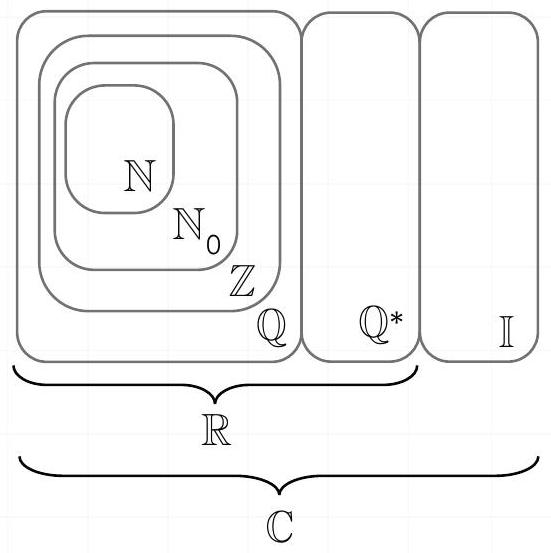
\includegraphics[max width=\textwidth, alt={}, center]{6dac6155-c874-45cc-9ccc-317741928334-003_553_551_366_1610}

Números Complejos $\mathbb{C}$. Ejemplos: $\{1,-i, 3+2 i, 1-i, \ldots\}$\\
a. Números enteros

Los números enteros $\mathbb{Z}$, incluyen a los números naturales, a los opuestos de estos y al cero. Estos se representan en la recta numérica horizontal, quedando los positivos a la derecha del cero y los negativos a la izquierda.\\
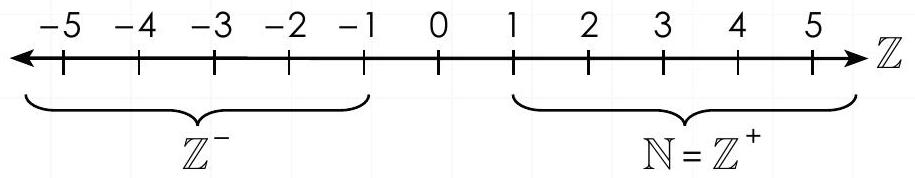
\includegraphics[max width=\textwidth, alt={}, center]{6dac6155-c874-45cc-9ccc-317741928334-003_178_915_1285_925}

El conjunto de los números enteros es un conjunto ordenable y, por lo mismo, podemos comparar sus valores y decidir si dos números enteros son iguales o distintos, y si son distintos, cuál de ellos es el mayor y cuál es el menor.

\section*{b. Valor absoluto}
El valor absoluto de un número x se escribe $|\mathbf{x}|$ y su valor corresponde a la distancia que existe entre el número x y el 0 . Así, el valor de $|x|$ es siempre mayor o igual a 0 , pues corresponde a una distancia y por tanto no puede ser negativo. Por ende, para cualquier valor real $x$, se tendrá que $|x| \geq 0$.

\begin{figure}[h]
\begin{center}
  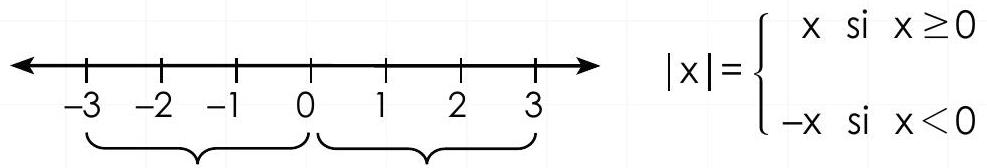
\includegraphics[alt={},max width=\textwidth]{6dac6155-c874-45cc-9ccc-317741928334-004_168_987_612_910}
\captionsetup{labelformat=empty}
\caption{$|-3|=3 \quad|3|=3$}
\end{center}
\end{figure}

\section*{TIP:}
Para cualquier par de valores a y b, siempre se cumple que: $|a-b|=|b-a|$.\\
Ejemplo: $|7-3|=|4|=4$ y $|3-7|=|-4|=4$

\section*{i. Propiedades del valor absoluto}
Para cualquier par de valores a y b, sus valores absolutos siempre cumplirán con las siguientes propiedades:

\section*{1. Multiplicación:}
$$
|a| \cdot|b|=|a \cdot b|
$$

Ejemplo: $|5| \cdot|-3|=|5 \cdot-3|=15$\\
2. División:

$$
\frac{|a|}{|b|}=\left|\frac{a}{b}\right|, \text { con } b \neq 0 .
$$

Ejemplo: $\frac{|6|}{|-2|}=\left|\frac{6}{-2}\right|=3$

\section*{3. Potencia:}
$$
\left|a^{n}\right|=|a|^{n}, \text { con } n \in \mathbb{Z} .
$$

Ejemplo: $\left|(-3)^{2}\right|=|-3|^{2}=9$

\section*{2. ORDEN EN EL CONJUNTO DE LOS NÚMEROS ENTEROS}
En el conjunto de los números enteros existe una relación de orden entre sus elementos y, por ende, los podemos ordenar de menor a mayor. Para esto utilizamos lo que se conoce como "Ley de Tricotomía", que señala que todo par de números, $x$ e $y$, deben cumplir con una de las siguientes condiciones:

\begin{itemize}
  \item " $x$ es menor que $y$ " y se escribe " $x<y$ ".
  \item " $x$ es igual a $y$ " y se escribe " $x=y$ ".
  \item " $x$ es mayor que $y$ " y se escribe " $x>y$ ".
\end{itemize}

Es en esta lógica comparativa que necesitamos tener algún mecanismo para ordenar a estos elementos. La forma más simple que tenemos para decidir entre dos números distintos cuál es el menor, es mirar su ubicación en la recta numérica, pues será menor aquel que esté más a la izquierda. No obstante lo anterior, también podemos decidir el orden entre dos o más números enteros a partir de su signo y su valor absoluto. Esto se reduce a:

\begin{itemize}
  \item Si a y $b$ son dos números enteros distintos y positivos, diremos que $a$ es menor que $b$, y escribiremos $a <\mathrm{b}$, cada vez que $|\mathrm{a}|<|\mathrm{b}|$.
\end{itemize}

Ejemplos: $\triangleright 8<10$, pues $|8|<|10| \quad \triangleright 25>9$, pues $|25|>|9|$

\begin{itemize}
  \item Si a y b son dos números enteros distintos y negativos, diremos que a es menor que b, y escribiremos $a<b$, cada vez que $|a|>|b|$.
\end{itemize}

Ejemplos: $\triangleright-3>-7$, pues $|-3|<|-7| \quad \triangleright-10<-9$, pues $|-10|>|-9|$

\begin{itemize}
  \item Si a y b son dos números enteros tales que $\boldsymbol{a}<\boldsymbol{0}$ y $\boldsymbol{>} \mathbf{0}$, siempre diremos que a es menor que b, independiente de su valor absoluto.
\end{itemize}

Ejemplos: $\quad \triangleright-8<10$, pues $-8<0$ y $10>0$ - $1>-190$, pues $1>0$ y $-190<0$

\section*{3. LAS CUATRO OPERACIONES BÁSICAS EN LOS ENTEROS}
a. Adición y Sustracción

Números de igual signo.

Para adicionar números de igual signo se deben sumar los valores absolutos de ellos conservando el signo común.

\section*{Números de distinto signo.}
Para adicionar números de distinto signo, primero determinamos los valores absolutos de cada número, y luego se resta el mayor menos el menor. Se conserva el signo del número cuyo valor absoluto sea mayor.

\section*{Ejemplos:}
$$
\begin{aligned}
& \triangleright \quad 5+7=12 \\
& \square \quad-5-7=-12
\end{aligned}
$$

\section*{Ejemplos:}
$$
\begin{aligned}
& \triangleright \quad 5-7=-2 \\
& \triangleright \quad-5+7=2
\end{aligned}
$$

Tener en cuenta que restar un valor es equivalente a sumar el opuesto de ese mismo valor. Esto es: $8-5=8+(-5)=3$

TIPS: Si tenemos que calcular una sustracción, se dará uno de los siguientes escenarios: »Siempre que a un número mayor le restamos uno menor, el resultado es un número positivo.

Ejemplos:

$$
\triangleright 7-5=2 \quad \triangleright 2-(-6)=8 \quad \triangleright-1-(-8)=7
$$

»Siempre que a un número menor le restamos uno mayor, el resultado es un número negativo.\\
Ejemplos:

$$
\triangleright 3-6=-3 \quad \triangleright-1-4=-5 \quad \triangleright-5-(-2)=-3
$$

\section*{b. Multiplicación y División}
\section*{Números de igual signo.}
Para multiplicar (o dividir) dos números de igual signo, se multiplican (o dividen) los respectivos valores absolutos de los números y el resultado siempre será positivo.

\section*{Ejemplos:}
\begin{itemize}
  \item $5 \cdot 7=35$
  \item $(-5) \cdot(-7)=35$
  \item $10: 2=5$
  \item $(-10):(-2)=5$
\end{itemize}

Números de distinto signo.

Para multiplicar (o dividir) dos números de distinto signo, se multiplican (o dividen) los valores absolutos de los números, y el resultado siempre será negativo.

\section*{Ejemplos:}
$$
\begin{array}{ll}
\triangleright & 5 \cdot(-7)=-35 \\
\triangleright & (-5) \cdot 7=-35 \\
\triangleright & 10:(-2)=-5 \\
\triangleright & (-10): 2=-5
\end{array}
$$

Regla de los signos en multiplicación y división de números.

\begin{center}
\begin{tabular}{|c|c|}
\hline
\begin{tabular}{c}
Números de \\
igual signo \\
\end{tabular} & \begin{tabular}{c}
Números de \\
igual signo \\
\end{tabular} \\
\hline
$+\cdot+=+$ & $+\cdot==-$ \\
\hline
$-\cdot==+$ & $-\cdot+=-$ \\
\hline
\end{tabular}
\end{center}

\begin{center}
\begin{tabular}{|c|c|}
\hline
\begin{tabular}{c}
Números de \\
igual signo \\
\end{tabular} & \begin{tabular}{c}
Números de \\
igual signo \\
\end{tabular} \\
\hline
$+:+=+$ & $+:-=-$ \\
\hline
$-:-=+$ & $-:+=-$ \\
\hline
\end{tabular}
\end{center}

\section*{4. MÚLTIPLOS Y DIVISORES}
\section*{a. Múltiplos}
Un número natural " $a$ " es un múltiplo de un número natural " $b$ ", si existe un $k \in \mathbb{N}$, tal que $a=k \cdot b$.

\section*{Ejemplos:}
\begin{itemize}
  \item 12 es múltiplo de 3 , porque existe $\mathrm{k}=4$, tal que $12=4 \cdot 3$.
  \item 28 es múltiplo de 4 , porque existe $\mathrm{k}=7$, tal que $28=7 \cdot 4$.
  \item 35 no es múltiplo de 4 , porque no existe un valor natural k , tal que $35=\mathrm{k} \cdot 4$.\\
¿Cuántos múltiplos tiene un número natural? La respuesta es: Infinitos. Por ejemplo para el 3, se tiene que:
\end{itemize}

$$
\text { Múltiplos de } 3=\{3,6,9,12,15,18, \ldots \text { etc }\}
$$

Pero los múltiplos ¿son solo valores positivos? La respuesta es NO, pues una vez que avanzamos de conjunto numérico al conjunto de los números enteros necesitamos ampliar el concepto a los múltiplos negativos - al propio cero, pues 0 es múltiplo de todo número entero. Así, podríamos pensar en que los múltiplos de 3 serán ahora:

$$
\text { Múltiplos de } 3=\{\text { etc., ......, }-18,-15,-12,-9,-6,-3,0,3,6,9,12,15,18, \ldots ., \text { etc. }\}
$$

\section*{b. Divisores}
Un número natural "b" es un divisor de un número natural "a", si al dividir "a" en "b" obtenemos como cociente un natural y un resto igual a cero.

\section*{Ejemplos}
\begin{itemize}
  \item 4 es divisor de 20 , porque $20: 4=5$ y su resto es 0 .
  \item 7 es divisor de 14 , porque $14: 7=2$ y su resto es 0 .
  \item 8 no es divisor de 15, porque $15: 8=1$, pero su resto es 7 .\\
¿Cuántos divisores tiene un número natural? Eso depende de cada número. Por ejemplo:
  \item Divisores de $10=\{1,2,5,10\}$, son 4 .
  \item Divisores de $24=\{1,2,3,4,6,8,12,24\}$, son 8 .
  \item Divisores de $5=\{1,5\}$
\end{itemize}

Según esta definición, todo número natural mayor que 1 tendrá al menos 2 divisores: el número 1 y el número mismo.\\
Igual que en el caso de los múltiplos, podríamos preguntarnos ¿́los divisores son solo valores positivos?. La respuesta es nuevamente NO, pues en el conjunto de los números enteros necesitamos ampliar el concepto a los divisores negativos. Así, podríamos pensar por ejemplo los divisores negativos de 8, que serían:

$$
\text { Divisores negativos de } 8=\{-8,-4,-2,-1\}
$$

Notemos también que 0 tiene infinitos divisores, pero que 0 no es divisor de ningún número.

\section*{5. PARIDAD E IMPARIDAD}
En el conjunto de los números enteros, se dice que un número es par, cada vez que se trate de un múltiplo de 2 . En caso contrario, diremos que ese número es impar.

\section*{Ejemplos}
\begin{itemize}
  \item Son pares: $28,-4,16,-400$, etc. (cualquier número entero que sea múltiplo de 2 ).
  \item Son impares: $17,-9,113,501$, etc. (todo número que no sea múltiplo de 2 ).
\end{itemize}

\section*{TIP:}
» Si bien el número 0 no es positivo ni negativo, sí es un número par.

Cada vez que operemos entre números pares e impares se dará alguna de las siguientes situaciones:\\
» La suma o resta de dos números pares, siempre nos dará como resultado un número par.\\
Ejemplos:

\begin{itemize}
  \item $2+4=6$
  \item $-14+8=-6$\\
» La suma o resta de dos números impares, siempre da como resultado un número par.\\
Ejemplos:
  \item $3+7=10$
  \item $11-5=6$\\
» La suma o resta de un número par y un impar, siempre da como resultado un número impar.\\
Ejemplos:
  \item $7+2=9$
  \item $16-5=11$\\
» La multiplicación de dos números pares, siempre da como resultado un número par.\\
Ejemplos:
  \item $8 \cdot 4=32$
  \item $10 \cdot-2=-20$\\
» La multiplicación de un número par y un impar siempre da como resultado un número par.\\
Ejemplos:
  \item $7 \cdot 4=28$
  \item $-4 \cdot-9=36$\\
» La multiplicación de dos números impares, siempre da como resultado un número impar.\\
Ejemplos:
  \item $7 \cdot 5=35$
  \item $-3 \cdot 9=-27$
\end{itemize}

\section*{6. PROPIEDADES DE LAS OPERACIONES EN LOS NÚMEROS ENTEROS}
a. Propiedad Conmutativa

La adición y la multiplicación en los enteros cumplen con la propiedad conmutativa, esto significa que el resultado es el mismo, independiente del orden en que se ubiquen los elementos en la operación. Es decir, si a y b son números enteros, se cumple que:

$$
\begin{aligned}
& a+b=b+a \text { Ejemplos: } a \cdot b=b \cdot a \\
\triangleright 5+6=11 \text { y } 6+5=11 & \triangleright 6 \cdot 7=42 \text { y } 7 \cdot 6=42 \\
\therefore 6+5=5+6 & \therefore 6 \cdot 7=7 \cdot 6
\end{aligned}
$$

b. Propiedad Asociativa

La adición y la multiplicación en los enteros cumplen con la propiedad asociativa, esto significa que el resultado es el mismo, independiente de cómo se agrupen inicialmente los elementos. Es decir, si a, b y c son números enteros, se cumple:

$$
a+(b+c)=(a+b)+c \text { y } a \cdot(b \cdot c)=(a \cdot b) \cdot c
$$

\section*{Ejemplos:}
$$
\begin{array}{lll}
\triangleright & (2+1)+6=3+6=9 & -\underline{-3 \cdot 2 \cdot 5}=-6 \cdot 5=-30 \\
2+(1+6)=2+7=9 & -3 \cdot 2 \cdot 5=-3 \cdot 10=-30 \\
\therefore(2+1)+6=2+(1+6) & \therefore-3 \cdot 2 \cdot 5=-3 \cdot 2 \cdot 5
\end{array}
$$

\section*{c. Propiedad Distributiva}
La multiplicación en los enteros cumple con la propiedad distributiva con respecto a la suma y a la resta. Es decir, si $a$, $b$ y $c$ son números enteros, se cumple:

$$
a \cdot(b+c)=a \cdot b+a \cdot c \text { y } a \cdot(b-c)=a \cdot b-a \cdot c
$$

Ejemplos:

$$
\begin{array}{ll}
\triangleright 3 \cdot(5+7)=3 \cdot(12)=36 & \triangleright 3 \cdot(2-7)=3 \cdot(-5)=-15 \\
\triangleright 3 \cdot 5+3 \cdot 7=15+21=36 & \triangleright 3 \cdot 2-3 \cdot 7=6-21=-15 \\
\therefore 3 \cdot(5+7)=3 \cdot 5+3 \cdot 7 & \therefore 3 \cdot(2-7)=3 \cdot 2-3 \cdot 7
\end{array}
$$

\section*{d. Neutro Aditivo y Neutro Multiplicativo}
Al sumar cualquier número entero a con 0 , el resultado es el mismo número $a$. Es decir, $a+0=a$ y $0+a=$ a. De hecho, se define al $\mathbf{0}$ como el elemento neutro aditivo.

Al multiplicar cualquier número entero a con 1, el resultado es el mismo número a. Es decir, $a \cdot 1=a$ y $1 \cdot a=a$. De hecho, se define al 1 como el elemento neutro multiplicativo.

\section*{Ejemplos:}
\begin{itemize}
  \item En el caso del neutro aditivo:
\end{itemize}

$$
0+4=4
$$

\begin{itemize}
  \item En el caso del neutro multiplicativo:
\end{itemize}

$$
1 \cdot 20=20
$$

\section*{e. Inverso Aditivo}
El inverso aditivo de a (con $a \neq 0$ ), es un número $b$ que sumado con a da como resultado 0 . Es decir, $b$ es el inverso aditivo de $a$ si $a+b=0$. Por lo tanto, $b=-a$ y denotamos al inverso aditivo de $a$ como $-a$.\\
Ejemplos:

\begin{itemize}
  \item Si el número es 5 , su inverso aditivo es -5 .
  \item Si el número es - 8 , su inverso aditivo es $-(-8)=8$.
\end{itemize}

\section*{f. Elemento Absorbente}
Si multiplicamos un número a con 0 , el resultado siempre será 0 . Es decir, $a \cdot 0=0$ y $0 \cdot a=0$, por lo tanto, se define al 0 como el elemento absorbente con la multiplicación.\\
Ejemplos:

$$
\begin{array}{ll}
\triangleright 0 \cdot 8=0 & \triangleright \pi \cdot 0=0 \\
\triangleright-7 \cdot 0=0 & \triangleright 0 \cdot 0=0
\end{array}
$$

\section*{g. Prioridad de las operaciones}
Cuando se requiere efectuar varias operaciones en un mismo ejercicio, se debe respetar el siguiente orden de las operaciones:

\begin{enumerate}
  \item Paréntesis, de adentro hacia afuera.
  \item Potencias y Raíces.
  \item Multiplicación y división (de izquierda a derecha).
  \item Adición y sustracción.
\end{enumerate}

\section*{Ejemplo:}
Resolver la siguiente operación:

$$
\begin{aligned}
& 8 \cdot(7-4): 12-1+6: 3 \cdot 9 \\
& =8 \cdot 3: 12-1+6: 3 \cdot 9 \\
& =24: 12-1+2 \cdot 9 \\
& =2-1+18 \\
& =19
\end{aligned}
$$

Nota: Esta regla también es conocida como PAPOMUDAS, que es la unión de las primeras letras de la prioridad de las operaciones: Paréntesis, Potencias y raíces, Multiplicación y División, Adición y Sustracción.

\section*{7. CRITERIOS DE DIVISIBILIDAD}
Para determinar de manera rápida si un número es divisible por otro número, podemos usar los criterios de divisibilidad. Un número será divisible por:\\
$\mathbf{2} \rightarrow$ Si su último dígito es par.

\section*{Ejemplo:}
$$
\triangleright \mathbf{2} ; \mathbf{1 4} ; \mathbf{2 7 8} ; \mathbf{2 . 4 3 0} \text {; etc. }
$$

$\mathbf{3} \rightarrow$ Si la suma de sus dígitos es múltiplo de $\mathbf{3}$.

\section*{Ejemplo:}
\begin{itemize}
  \item 234 es divisible por 3 , pues $2+3+4=9$
  \item 3.621 es divisible por 3, pues
\end{itemize}

$$
3+6+2+1=12
$$

$\mathbf{4} \rightarrow$ Si sus dos últimos dígitos forman un múltiplo de 4 o son ceros.

\section*{Ejemplo:}
$$
\triangleright \mathbf{2 4} ; 184 ; 1.300 ; 213.436 ; \text { etc. }
$$

$7 \rightarrow$ Si al multiplicar el dígito de las unidades por 2 y restándola al número formado por los otros dígitos, el resultado es un múltiplo de $7 \circ 0$.

\section*{Ejemplo:}
\begin{itemize}
  \item 896 es divisible por 7, pues al multiplicar 6 por 2, nos da 12, y si restamos 12 a 89 (el número que forman los otros dígitos), nos da 77, que es un múltiplo de 7.\\
$\mathbf{8} \rightarrow$ Si sus tres últimos dígitos forman un múltiplo de 8 o son ceros.
\end{itemize}

\section*{Ejemplo:}
\begin{itemize}
  \item 21.936 es divisible por 8, pues 936 (el número formado por sus últimos 3 dígitos) es un múltiplo de 8.\\
$\mathbf{5} \rightarrow$ Si termina en 0 o 5.
\end{itemize}

\section*{Ejemplo:}
\begin{itemize}
  \item $20 ; 385 ; 1.340 ; 762.435$; etc.\\
$\mathbf{6} \rightarrow$ Si es divisible por 2 y 3 a la vez.\\
Ejemplo:
  \item 1.350 es divisible por 6, pues termina en 0 (par), por lo que es divisible por 2 , y $1+3+5+0=9$, que es múltiplo de 3 , por lo que también es divisible por 3.
\end{itemize}

9 → Si la suma de sus dígitos es múltiplo de 9 .

\section*{Ejemplo:}
\begin{itemize}
  \item 5.643 es divisible por 9, pues $5+6+4+3=18$, que es un múltiplo de 9 .\\
$\mathbf{1 0} \boldsymbol{\rightarrow}$ Si su último dígito es 0.
\end{itemize}

\section*{Ejemplo:}
\begin{itemize}
  \item 23.140 es divisible por 10 , pues es un número terminado en 0 .
\end{itemize}

\section*{Ejemplos}
\begin{enumerate}
  \item ¿Cuál es el valor de $1-(-3)(-2-6)$ ?
\end{enumerate}

HABILIDAD: RESOLVER PROBLEMAS. (DEMRE 2026)\\
A) -32\\
B) -23\\
C) -16\\
D) -4\\
2. La temperatura en una cámara de frigorífico es de $12^{\circ} \mathrm{C}$. Se necesita variar esta temperatura hasta alcanzar los $-36^{\circ} \mathrm{C}$. Si la temperatura desciende $3^{\circ} \mathrm{C}$ cada cinco minutos, ¿cuánto tiempo se tardará en alcanzar dicha temperatura?\\
HABILIDAD: RESOLVER PROBLEMAS. (DEMRE 2024)\\
A) 85 minutos.\\
B) 80 minutos.\\
C) 60 minutos.\\
D) 48 minutos.\\
3. Si la suma de 3 números enteros consecutivos es igual a p, ¿cuál de las siguientes afirmaciones es siempre verdadera respecto al valor de p?\\
HABILIDAD: ARGUMENTAR. (DEMRE 2024)\\
A) Es un número impar.\\
B) Es un múltiplo de 3.\\
C) Es un número positivo.\\
D) Es un número distinto de cero.\\
4. Considera la siguiente recta numérica:\\
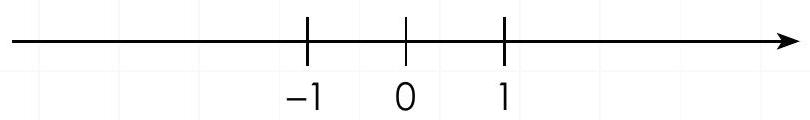
\includegraphics[max width=\textwidth, alt={}, center]{6dac6155-c874-45cc-9ccc-317741928334-024_120_810_312_937}\\
¿Cuál de los siguientes procedimientos representa la operación $-5+(-8)$ usando la recta numérica? HABILIDAD: REPRESENTAR. (DEMRE 2025)\\
A) Ubicarse en el -5 y desplazarse 8 unidades a la izquierda.\\
B) Ubicarse en el -5 y desplazarse 8 unidades a la derecha.\\
C) Ubicarse en el -8 y desplazarse 5 unidades a la derecha.\\
D) Ubicarse en el -8 y desplazarse 3 unidades a la derecha.\\
5. ¿Cuántos números enteros positivos son mayores o iguales que -4 y menores que 3 ?

HABILIDAD: RESOLVER PROBLEMAS. (DEMRE 2025)\\
A) 2\\
B) 3\\
C) 4\\
D) 6

\section*{8. NÚMEROS PRIMOS, COMPUESTOS Y TEOREMA FUNDAMENTAL}
Números primos son aquellos números enteros positivos mayores que uno, que tienen exactamente dos divisores positivos y distintos entre sí. Los primeros números primos son:

$$
2,3,5,7,11,13,17,19,23,29,31,37, \ldots
$$

Números compuestos son todos los números enteros positivos mayores que uno, que no son primos. Los primeros números compuestos son: $4,6,8,9,10,12,14,15,16,18,20,21,22, \ldots$\\
El teorema fundamental de la aritmética establece que todo número natural mayor que uno se puede expresar de manera única como el producto de potencias con números primos en sus bases. Para realizar esta descomposición podemos utilizar la tabla de descomposición o bien el diagrama de árbol.

\begin{displayquote}
» Nota: La cantidad total de divisores positivos que tenga el número estará dada por el producto de los sucesores de los exponentes de dicha descomposición.
\end{displayquote}

\section*{i. Tabla de descomposición}
La tabla funciona dividiendo al número compuesto por números primos hasta que quede reducido a la unidad.

\section*{ii. Diagrama de árbol}
El diagrama de árbol es un método más intuitivo. Comienza expresando el número como el producto de dos números cualesquiera, luego estos números se vuelven a descomponer hasta que en las ramas solo queden números primos.

\section*{Ejemplo:}
\begin{itemize}
  \item Hallar la descomposición prima de 90.\\
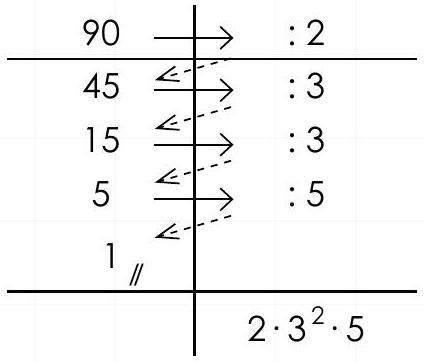
\includegraphics[max width=\textwidth, alt={}, center]{6dac6155-c874-45cc-9ccc-317741928334-027_362_424_412_620}\\
∴ La descomposición prima de 90 es $2 \cdot 3^{2} \cdot 5$.
\end{itemize}

\section*{Ejemplo:}
\begin{itemize}
  \item Hallar la descomposición prima de 90.\\
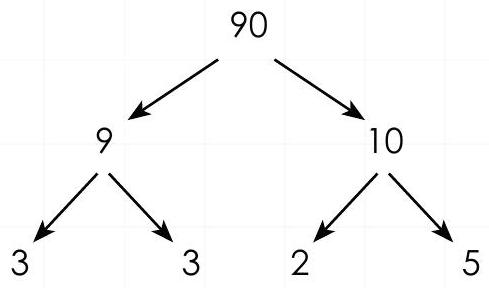
\includegraphics[max width=\textwidth, alt={}, center]{6dac6155-c874-45cc-9ccc-317741928334-027_288_489_406_1493}\\
∴ La descomposición prima de 90 es $2 \cdot 3^{2} \cdot 5$.
  \item Total de divisores de $90: 2^{1} \cdot 3^{2} \cdot 5^{1} \rightarrow(1+1)(2+1)(1+1) \Rightarrow 2 \cdot 3 \cdot 2 \Rightarrow 12$
  \item Esto quiere decir que 90 tiene 12 divisores: $\{1,2,3,5,6,9,10,15,18,30,45,90\}$
\end{itemize}

\section*{TIPS:}
» El menor número primo es el 2, el que además es el único número primo que es par.\\
» El 1 no es primo ni compuesto.

\section*{9. MÍNIMO COMÚN MÚLTIPLO (m.c.m) Y MÁXIMO COMÚN DIVISOR (M.C.D)}
a. Mínimo común múltiplo (m.c.m)

El mínimo común múltiplo (m.c.m) de dos o más números, es el menor entero positivo que es múltiplo común de dichos números. A continuación se muestran dos métodos para obtener el mínimo común múltiplo. Estos son: la tabla de descomposición y la descomposición prima.

\section*{i. Tabla de descomposición}
Hacer una tabla en la cual dos o más números se van dividiendo por números primos (algunos de ellos pueden ser comunes) hasta que cada número queda totalmente descompuesto. El m.c.m será la multiplicación de los factores primos.

\section*{ii. Descomposición prima}
Desarrollar la descomposición prima de todos los números y multiplicar todos los factores primos distintos que aparezcan, elevados cada uno al mayor exponente que tenga en las descomposiciones.

\section*{Ejemplo:}
\begin{itemize}
  \item Sean $\mathrm{A}=90$ y $\mathrm{B}=24$, determinar el m.c.m.
\end{itemize}

\begin{center}
\begin{tabular}{cc|c}
24 & 90 & $: 2$ \\
\hline
12 & 45 & $: 2$ \\
6 & 45 & $: 2$ \\
3 & 45 & $: 3$ \\
$1 / /$ & 15 & $: 3$ \\
 & 5 & $: 5$ \\
 & $1 / /$ &  \\
\hline
 & m.c.m $=$ & $2^{3} \cdot 3^{2} \cdot 5$ \\
\hline
\end{tabular}
\end{center}

$\therefore \quad$ el m.c.m entre 90 y 24 es $2^{3} \cdot 3^{2} \cdot 5$.

\section*{Ejemplo:}
\begin{itemize}
  \item Sean $\mathrm{A}=90$ y $\mathrm{B}=24$, determinar el m.c.m.
\end{itemize}

$$
A=2 \cdot 3^{2} \cdot 5 \text { y } B=2^{3} \cdot 3
$$

$\therefore \quad$ el m.c.m entre 90 y 24 es $2^{3} \cdot 3^{2} \cdot 5$.\\
b. Máximo común divisor (M.C.D)

El máximo común divisor (M.C.D) de dos o más números, es el mayor entero positivo que es divisor común de dichos números. A continuación se muestran dos métodos para obtener el máximo común divisor. Estos son: la tabla de descomposición y la descomposición prima.

\section*{i. Tabla de descomposición}
Hacer una tabla en la cual dos o más números se van dividiendo por números primos comunes hasta que no exista otro número primo que pueda dividir a ambos números. El M.C.D será la multiplicación de los factores primos.

\section*{Ejemplo}
\begin{itemize}
  \item Sean $\mathrm{A}=90$ y $\mathrm{B}=24$, determinar el M.C.D
\end{itemize}

\begin{center}
\begin{tabular}{cc|c}
24 & 90 & $: 2$ \\
\hline
12 & 45 & $: 3$ \\
4 & 15 &  \\
\hline
 & M.C.D $=$ & $2 \cdot 3$ \\
\hline
\end{tabular}
\end{center}

$\therefore$ el M.C.D entre 90 y 24 es $2 \cdot 3$.

\section*{ii. Descomposición prima}
Desarrollar la descomposición prima de todos los números y multiplicar solo los factores primos comunes que aparezcan en los números, elevados cada uno al menor exponente que tenga en las descomposiciones.

\section*{Ejemplo:}
\begin{itemize}
  \item Sean $\mathrm{A}=90$ y $\mathrm{B}=24$, determinar el M.C.D
\end{itemize}

$$
A=2 \cdot 3^{2} \cdot 5 \text { y } B=2^{3} \cdot 3
$$

$\therefore$ el M.C.D entre 90 y 24 es $2 \cdot 3$.\\
» Nota. Los números que no tienen factores primos comunes se denominan primos relativos entre sí.\\
En tal caso se cumple que el m.c.m es el producto de los números y el M.C.D será siempre 1.\\
Por ejemplo, 9 y 10 son primos relativos entre sí, ya que los factores primos de 9 son $\{3,3\}$, y los factores primos de 10 son $\{2,5\}$. Por tanto: el m.c.m entre 9 y 10 es 90 , el M.C.D entre 9 y 10 es 1 .

\section*{c. Problemas de aplicación}
Las aplicaciones de el m.c.m. y el M.C.D. que frecuentemente nos podremos encontrar:

\section*{Ejemplos:}
\begin{itemize}
  \item En el baño de un colegio hay 3 llaves de agua cerradas. Estas se encuentran en mal estado, y gotean constantemente cada cierto tiempo. La llave A deja caer una gota cada 3 segundos; la llave B lo hace cada 5 segundos y, la llave C, cada 8 segundos. Si en un instante las 3 llaves dejaron caer una gota al mismo tiempo, ¿cuántos segundos deben transcurrir a partir de ese momento, para que vuelvan a coincidir nuevamente?
\end{itemize}

\section*{Solución:}
Para resolver este problema, debemos considerar que la llave A gotea a partir de ese instante a los 3 segundos, luego a los 6 segundos, a los 9, 12, 15, etc. Es decir, son los múltiplos de 3 (en segundos). Por su parte, la llave B lo hará a los $5,10,15,20$, etc. (los múltiplos de 5 ) y, por la misma razón, la llave C lo hará en los múltiplos de 8 . Por lo tanto, las llaves coincidirán nuevamente en una cantidad de segundos que sea múltiplo de 2 , de 3 y de 8 ; es decir, en un múltiplo común de estos 3 números. Y si queremos que sea lo antes posible, debemos determinar por ello el mínimo común múltiplo de 3,5 y 8, que es 120.\\
Con todo lo anterior, podemos contestar que, 120 son los segundos que deben transcurrir para que estas llaves vuelvan a dejar caer una gota al mismo instante.

\begin{itemize}
  \item Una constructora necesita subdividir dos terrenos que están separados por un río y cuyas áreas son $21.600 \mathrm{~m}^{2}$ el más pequeño y $32.000 \mathrm{~m}^{2}$ el más grande. Esta constructora necesita además que estos terrenos más pequeños sean todos del mismo tamaño; que sea una cantidad entera de metros cuadrados y que sean lo más grandes posible, porque esto aumentará su valor comercial. ¿Cuál será el área máxima de estos terrenos si se cumple con la solicitud de esta empresa constructora?
\end{itemize}

\section*{Solución:}
En este caso, necesitamos dividir estos terrenos en terrenos más pequeños de igual área (digamos $\mathrm{X} \mathrm{m}^{2}$ ). Esto significa que tanto 21.600 como 32.000 deben ser divisibles por X o , lo que es lo mismo, X debe ser divisor tanto de 21.600 , como de 32.000 . Si además se exige que $X$ sea lo más grande posible, estamos hablando del máximo común divisor de 21.600 y 32.000 , que es 800 . Por lo tanto, cada terreno será de $800 \mathrm{~m}^{2}$ y habrán 27 de estos terrenos en el terreno más pequeño y 40 en el más grande.

\section*{10. EVALUAR EXPRESIONES}
Evaluar o valorizar una expresión algebraica consiste en sustituir las letras por los valores numéricos dados, y luego realizar las operaciones indicadas.\\
Ejemplos:

\begin{itemize}
  \item Si $m=-4$ y $n=-1$, entonces el valor de la expresión $m n-m^{2}$ es:
\end{itemize}

$$
\begin{aligned}
m n-m^{2} & =(-4)(-1)-(-4)^{2} \\
& =4-16 \\
& =-12
\end{aligned}
$$

»TIP. AI sustituir, conviene siempre incluir paréntesis, ya que así se reduce la probabilidad de llegar a un resultado incorrecto al no considerar el signo de los números evaluados.

\section*{11. ENUNCIADOS FRECUENTES}
Sean $x$ e y números enteros, entonces la transcripción matemática de los siguientes enunciados:

\section*{Expresiones}
\begin{itemize}
  \item El doble de x es 2x.
  \item El triple de x es 3x.
  \item La semisuma de x e y es $\frac{\mathbf{x + y}}{\mathbf{2}}$.
  \item El exceso de x sobre y es $\mathrm{x}-\mathrm{y}$.
  \item La mitad de $x$ es $\frac{\mathbf{1}}{\mathbf{2}} x \circ \frac{\mathbf{x}}{\mathbf{2}}$.
  \item El sucesor de x es ( $\mathrm{x}+1$ ).
  \item El antecesor de x es $(\mathrm{x}-1)$.
  \item Un número par es $\mathbf{2 x}$, siendo x un valor entero.
  \item Un número impar es $(2 x-1) \circ(2 x+1)$, siendo x un valor entero.
  \item Dos pares consecutivos son 2 x y $2 \mathrm{x}+2$.
\end{itemize}

\section*{Ejemplos:}
El doble de 3 es 6, pues $2 \cdot 3=6$.\\
El triple de -8 es -24 , pues $3 \cdot-8=-24$.\\
La semisuma de 4 y 12 es $8, \frac{4+12}{2}=8$.\\
El exceso de 8 sobre 3 es 5, pues $8-3=5$.\\
La mitad de 200 es 100, pues $\frac{200}{2}=100$.\\
El sucesor de -12 es -11 , pues $-12+1=-11$.\\
El antecesor de -4 es -5 , pues $-4-1=-5$.\\
14 es par, pues $14=2 \cdot 7$.

19 es impar, pues $2 \cdot 10-1=19 \circ 2 \cdot 9+1=19$.

10 y 12 son pares consecutivos, pues $2 \cdot 5=10$ y $2 \cdot 5+2=12$.

\section*{Expresiones}
\begin{itemize}
  \item Dos impares consecutivos son $2 x+1 y \mathbf{2 x} \boldsymbol{+} \mathbf{3} \boldsymbol{.}$
  \item El cuadrado de $x$ es $x^{2}$.
\end{itemize}

\section*{Ejemplos:}
7 y 9 son impares consecutivos, pues $2 \cdot 3+1$ y $2 \cdot 3+3$.

El cuadrado de 5 es 25 , pues $5^{2}=5 \cdot 5=25$.

\section*{Ejemplos}
\begin{enumerate}
  \setcounter{enumi}{5}
  \item En la siguiente infografía se presenta el pronóstico del tiempo para cierto día, con la temperatura en grados Celsius.
\end{enumerate}

\begin{center}
\begin{tabular}{|l|l|l|l|l|}
\hline
\multicolumn{5}{|c|}{Ahora
\includegraphics[max width=\textwidth, alt={}]{6dac6155-c874-45cc-9ccc-317741928334-037_109_281_481_1222}
} \\
\hline
Resumen & Precipitaciones & Viento &  & Humedad \\
\hline
15:00 & 17:00 & 18:00 & 20:00 & 21:00 \\
\hline
$30^{\circ}$ & $29^{\circ}$ & $28^{\circ}$ & $26^{\circ}$ & $24^{\circ}$ \\
\hline
\end{tabular}
\end{center}

¿Cuál será la variación de temperatura entre las 17:00 y las 21:00 horas?\\
HABILIDAD: RESOLVER PROBLEMAS. (DEMRE 2025)\\
A) $-6^{\circ} \mathrm{C}$\\
B) $-5^{\circ} \mathrm{C}$\\
C) $4^{\circ} \mathrm{C}$\\
D) $6^{\circ} \mathrm{C}$\\
7. Si al quíntuplo de -10 se le resta el triple de -12 , ¿qué número se obtiene?

HABILIDAD: RESOLVER PROBLEMAS. (DEMRE 2024)\\
A) -86\\
B) -14\\
C) 2\\
D) 34\\
8. Una persona selecciona un número de dos dígitos, luego resta este número a 200 y , finalmente, duplica el resultado. ¿Cuál es el mayor número que puede obtener mediante esta serie de operaciones?\\
HABILIDAD: RESOLVER PROBLEMAS. (DEMRE 2024)\\
A) 220\\
B) 301\\
C) 380\\
D) 398\\
9. La automotora "Mi auto" tiene cinco marcas de automóviles, cada marca tiene tres modelos y cada modelo está en tres colores distintos.\\
La automotora "Viaje feliz" tiene cuatro marcas de automóviles, cada marca tiene tres modelos y cada modelo en cuatro colores distintos.

Si las marcas de los automóviles de las automotoras son distintas entre sí, ¿cuál de las siguientes afirmaciones es verdadera?

HABILIDAD: ARGUMENTAR. (DEMRE 2023)\\
A) La automotora "Viaje feliz" ofrece tres posibilidades distintas más para elegir un automóvil que la automotora "Mi auto".\\
B) Ambas automotoras ofrecen la misma cantidad de posibilidades distintas para elegir un automóvil.\\
C) La automotora "Mi auto" ofrece más posibilidades distintas para elegir un automóvil que la automotora "Viaje feliz".\\
D) El total de las distintas posibilidades de elegir un automóvil está determinado por la suma entre la cantidad de marcas, de modelos y de colores.\\
10. Un diario tiene una colilla recortable para un concurso, la que se presenta a continuación:

\section*{CUADRO MÁGICO}
\begin{center}
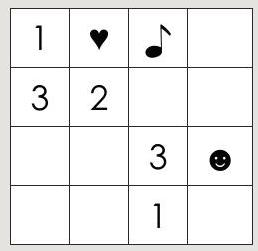
\includegraphics[max width=\textwidth, alt={}]{6dac6155-c874-45cc-9ccc-317741928334-041_251_258_385_945}
\end{center}

Cada fila, cada columna y cada diagonal deben contener los números 1, 2, 3 y $4 \sin$ que se repitan.

Manda el resultado correcto de\\

\includegraphics[max width=\textwidth, alt={}, center]{6dac6155-c874-45cc-9ccc-317741928334-041_51_176_418_1527}\\
a la casilla postal de este diario para entrar al concurso de una bicicleta\\
□\\
Resultado\\
Nombre $\_\_\_\_$ Número contacto $\_\_\_\_$\\
¿Cuál es el resultado que permite entrar al concurso?\\
HABILIDAD: RESOLVER PROBLEMAS. (DEMRE 2024)\\
A) 6\\
B) 7\\
C) 8\\
D) 9\\
11. Una empresa decide registrar mensualmente la variación de la masa total de los metales almacenados en su bodega. El primer mes aumentó en 2 toneladas la masa almacenada, en el segundo mes disminuyó en 4 toneladas la masa almacenada, el tercer mes aumentó en 3 toneladas la masa almacenada y el cuarto mes aumentó en 1 tonelada la masa almacenada. Al finalizar el cuarto mes la masa total de los metales en la bodega es de 70 toneladas.\\
Del departamento de ventas de la empresa necesitan saber la cantidad de toneladas de metal que había antes de comenzar los registros para completar el registro.\\
¿Cuántas toneladas de metal había almacenadas inicialmente en la bodega?\\
HABILIDAD: RESOLVER PROBLEMAS. (DEMRE 2024)\\
A) 66 toneladas.\\
B) 68 toneladas.\\
C) 70 toneladas.\\
D) 74 toneladas.\\
12. En la figura se presenta un cartel con los precios de las impresiones en blanco y negro de un centro de impresión.

\section*{IMPRESIONES B Y N}
\begin{table}[h]
\begin{center}
\captionsetup{labelformat=empty}
\caption{Lista de precios}
\begin{tabular}{cc}
Cantidad de hojas & Precio por hoja \\
de 1 a 99 hojas & $\$ 30$ \\
de 100 a 149 hojas & $\$ 25$ \\
150 o más & $\$ 20$ \\
\end{tabular}
\end{center}
\end{table}

Un curso de Química Orgánica requiere de un libro de tres capítulos de 150,130 y 85 hojas, en ese orden. Una persona imprimió primero solo el primer capítulo, luego solo el segundo y por último solo el tercero, a medida que avanzaba en el curso.\\
¿Cuánto dinero gastó la persona en imprimir el libro?\\
HABILIDAD: RESOLVER PROBLEMAS. (DEMRE 2024)\\
A) $\$ 7.300$\\
B) $\$ 8.150$\\
C) $\$ 8.800$\\
D) $\$ 9.450$\\
13. Consuelo y dos amigas comieron en un restaurante. A continuación se presenta la boleta de todo lo consumido por las tres amigas.

\begin{center}
\begin{tabular}{|crr|}
\hline
\multicolumn{3}{|c|}{Donde Nemesio} \\
******************************* &  &  \\
Cant. Item & Total &  \\
******************************* &  &  \\
1 & Jugo & $\$ 1.600$ \\
3 & Sándwich & $\$ 18.000$ \\
1 & Promoción & $\$ 4.800$ \\
2 & sopaipillas &  \\
Bebidas & $\$ 2.600$ &  \\
\multicolumn{3}{|l|}{*******************************} \\
Total &  & $\$ 27.000$ \\
\hline
\end{tabular}
\end{center}

Acordaron que cada una de ellas pagará lo que consumió y, además, la promoción de sopaipillas la dividirán en tres partes iguales y cada una pagará una de esas tres partes.

Si Consuelo consumió un sándwich y una bebida, ¿cuánto tiene que pagar?\\
HABILIDAD: RESOLVER PROBLEMAS. (DEMRE 2026)\\
A) $\$ 8.900$\\
B) $\$ 9.000$\\
C) $\$ 12.000$\\
D) $\$ 22.200$\\
14. Una persona realiza un viaje al exterior y lleva consigo su tarjeta de débito, la que funciona fuera del país. En su tarjeta tiene un saldo inicial de $\$ 300.000$ y decide hacer algunas actividades turísticas, por lo que realizó los siguientes movimientos en su tarjeta:

\begin{itemize}
  \item Un pago de \$15.000 para pagar la entrada a una obra de teatro.
  \item Un pago de \$35.000 para pagar el ingreso al parque de diversiones y algo de comida dentro del parque.
\end{itemize}

Si por cada pago que realiza con su tarjeta el banco le cobra una comisión de $\$ 2.000$ independientemente del monto, ¿cuál es su saldo final luego de realizados los pagos de ese día?

HABILIDAD: RESOLVER PROBLEMAS. (DEMRE 2024)\\
A) $\$ 254.000$\\
B) $\$ 244.000$\\
C) $\$ 248.000$\\
D) $\$ 246.000$\\
15. Dos personas se juntan a realizar ejercicios, pero cada una tiene su propia rutina, las que se detallan a continuación:

\begin{itemize}
  \item La primera persona realiza ejercicios durante 2 minutos y luego se toma 30 segundos de descanso, repitiendo esta serie ocho veces.
  \item La segunda persona realiza ejercicios durante 1 minuto y 30 segundos y luego se toma 15 segundos de descanso, repitiendo esta serie doce veces.
\end{itemize}

Si las dos personas comienzan sus rutinas al mismo tiempo, ¿cuál de los siguientes argumentos garantiza que una de las personas termina la rutina antes que la otra?

HABILIDAD: ARGUMENTAR. (DEMRE 2025)\\
A) Que la cantidad de repeticiones de las series de ambas personas es distinta.\\
B) Que el tiempo de descanso de ambas personas es distinto.\\
C) Que la suma entre el tiempo de ejercicio, el descanso y las repeticiones de las series es distinta en cada persona.\\
D) Que la suma entre el tiempo de ejercicio y el descanso, multiplicada por las repeticiones de las series, es distinta en cada persona.\\
16. Considera la siguiente secuencia de figuras:

\begin{figure}[h]
\begin{center}
  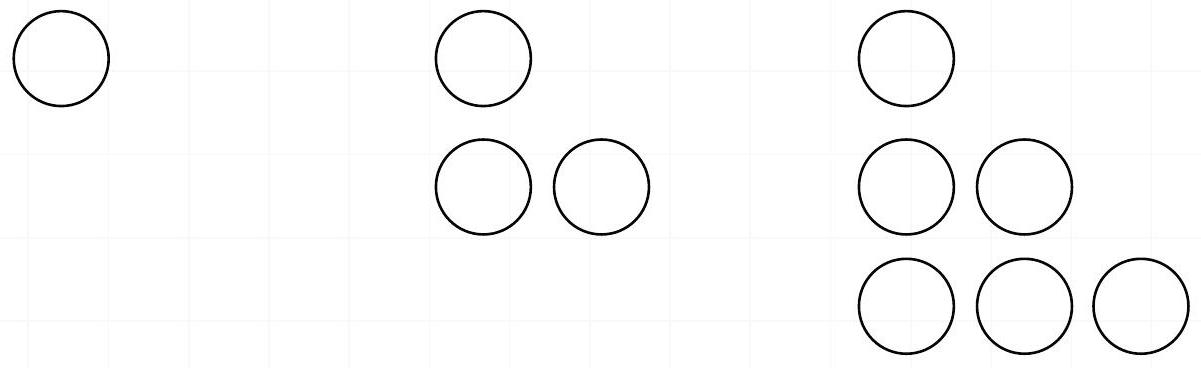
\includegraphics[alt={},max width=\textwidth]{6dac6155-c874-45cc-9ccc-317741928334-047_368_1201_312_787}
\captionsetup{labelformat=empty}
\caption{Figura 1}
\end{center}
\end{figure}

Figura 2

Figura 3

Si el patrón de formación se mantiene, ¿cuántos círculos forman la Figura 7?\\
HABILIDAD: RESOLVER PROBLEMAS. (DEMRE 2025)\\
A) 18\\
B) 21\\
C) 28\\
D) 36\\
17. Considera la siguiente secuencia de figuras, formadas por cuadrados y triángulos, que se va formando con palitos de fósforo.

\begin{figure}[h]
\begin{center}
\captionsetup{labelformat=empty}
\caption{Figura 1}
  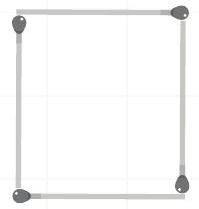
\includegraphics[alt={},max width=\textwidth]{6dac6155-c874-45cc-9ccc-317741928334-048_209_199_454_608}
\end{center}
\end{figure}

\begin{figure}[h]
\begin{center}
\captionsetup{labelformat=empty}
\caption{Figura 2}
  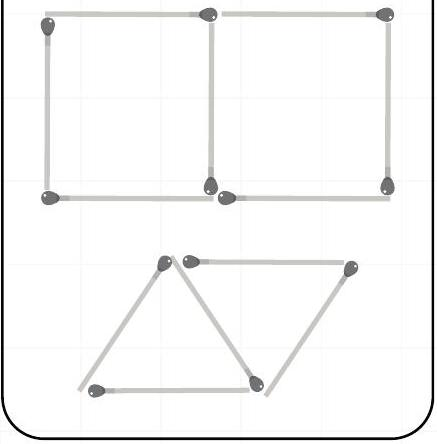
\includegraphics[alt={},max width=\textwidth]{6dac6155-c874-45cc-9ccc-317741928334-048_444_437_452_895}
\end{center}
\end{figure}

\begin{figure}[h]
\begin{center}
\captionsetup{labelformat=empty}
\caption{Figura 3}
  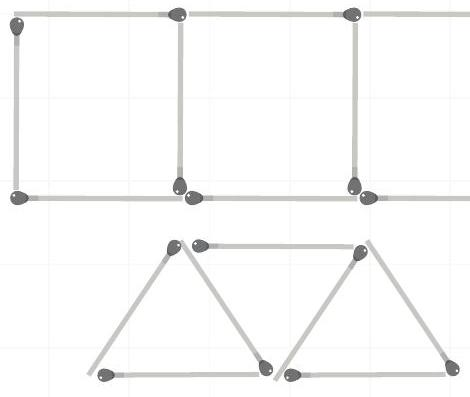
\includegraphics[alt={},max width=\textwidth]{6dac6155-c874-45cc-9ccc-317741928334-048_397_470_452_1408}
\end{center}
\end{figure}

⋯\\
¿Cuál es la cantidad de palitos que se utilizan en la figura 25?\\
HABILIDAD: REPRESENTAR. (DEMRE 2025)\\
A) $7 \cdot 25$\\
B) $5 \cdot 25+2$\\
C) $3 \cdot 25+4$\\
D) $2 \cdot 25$\\
18. Un juego consiste en lanzar cinco bolitas desde cierta distancia hacia los agujeros de una caja. Los puntajes se asignan según el agujero por el cual entra la bolita, como se presenta a continuación:\\
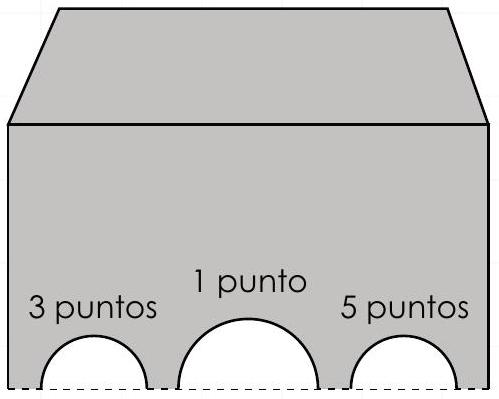
\includegraphics[max width=\textwidth, alt={}, center]{6dac6155-c874-45cc-9ccc-317741928334-049_399_499_370_1095}

Cuando una bolita no ingresa en alguno de los agujeros, se repite el lanzamiento. El juego finaliza cuando todas las bolitas entran por uno de los agujeros, siendo el puntaje final la suma de los puntajes asignados por donde ingresó cada una de las bolitas.

Una persona jugó este juego y se sabe que las bolitas ingresaron por los tres agujeros.\\
¿Cuál de los siguientes puntajes corresponde al máximo puntaje que pudo haber obtenido la persona al finalizar el juego?

HABILIDAD: RESOLVER PROBLEMAS. (DEMRE 2025)\\
A) 5\\
B) 11\\
C) 19\\
D) 25\\
19. En el gráfico adjunto se representa la percepción ciudadana en relación con los atributos de un candidato. Esta percepción se presenta en un puntaje que va de -20 a 20 puntos.\\
HABILIDAD: REPRESENTAR. (DEMRE 2026)\\
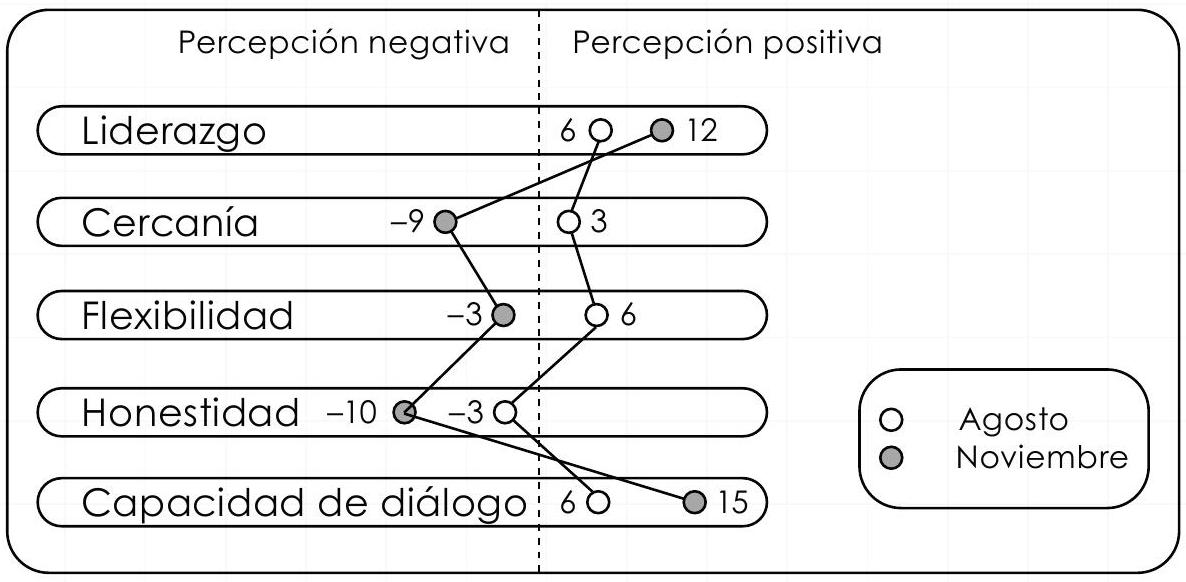
\includegraphics[max width=\textwidth, alt={}, center]{6dac6155-c874-45cc-9ccc-317741928334-050_582_1186_379_750}\\
¿Cuál de los atributos presentó una mayor variación en su puntaje según la percepción ciudadana, entre agosto y noviembre?\\
A) Liderazgo.\\
B) Cercanía.\\
C) Honestidad.\\
D) Capacidad de diálogo.\\
20. La masa molar de un compuesto químico se calcula sumando las masas molares de todos los átomos que lo conforman.\\
Considera el compuesto denominado ácido sulfúrico y la información que se presenta a continuación:\\
HABILIDAD: REPRESENTAR. (DEMRE 2026)\\
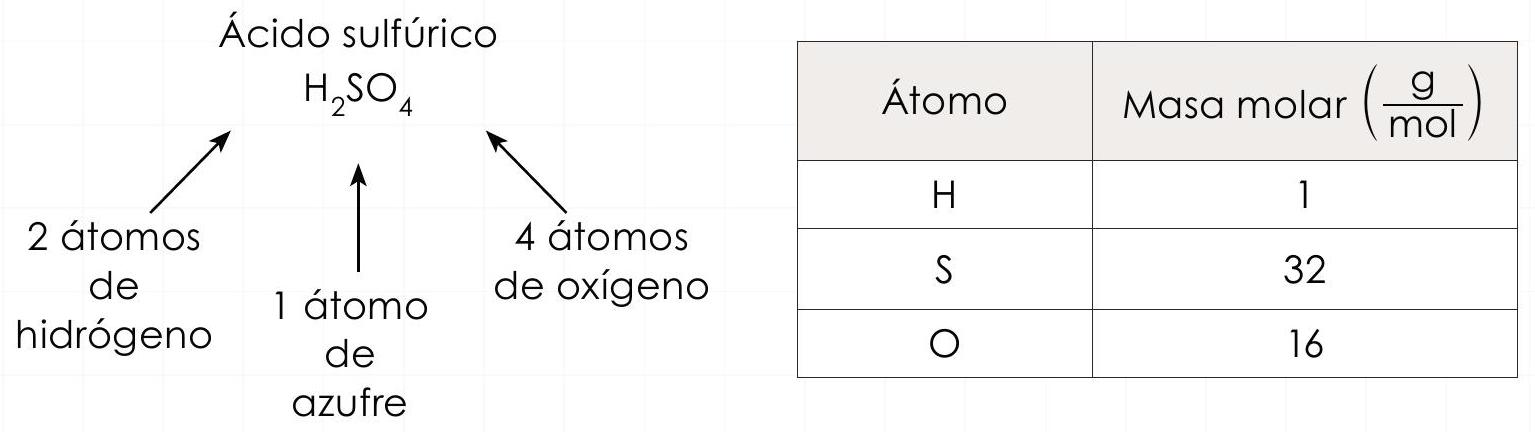
\includegraphics[max width=\textwidth, alt={}, center]{6dac6155-c874-45cc-9ccc-317741928334-051_432_1535_425_572}\\
¿Cuál de las siguientes expresiones representa la masa molar del ácido sulfúrico?\\
A) $(1+32+16) \frac{\mathrm{g}}{\mathrm{mol}}$\\
B) $(2+4) \cdot(32+16) \frac{\mathrm{g}}{\mathrm{mol}}$\\
C) $(2 \cdot 1+1 \cdot 32+4 \cdot 16) \frac{\mathrm{g}}{\mathrm{mol}}$\\
D) $(1+2+4) \cdot(1+32+16) \frac{\mathrm{g}}{\mathrm{mol}}$

\section*{Z Preuniversitario Zenit}
\section*{EJERCICIOS M1}
\begin{enumerate}
  \item $6-3 \cdot 8-32: 4=$\\
A) -26\\
B) -14\\
C) 0\\
D) 3
  \item $[-5+(-3) \cdot 7]:(-2)=$\\
A) 24\\
B) 13\\
C) -24\\
D) -13
  \item $-3 \cdot|6-8|-|-2|=$\\
A) -8\\
B) -4\\
C) 0\\
D) 4
  \item $(1+5)-3^{2}+8: 2 \cdot 2=$\\
A) -1\\
B) 1\\
C) 5\\
D) 15
  \item $76.606-29.878=$\\
A) 45.728\\
B) 46.728\\
C) 45.738\\
D) 46.736
  \item Si al entero ( -1 ) le restamos el entero ( -4 ), resulta:\\
A) 0\\
B) -3\\
C) 2\\
D) 3
  \item $-(4-2 \cdot(2-4))=$\\
A) -15\\
B) -10\\
C) -8\\
D) 8
  \item Si $\mathrm{M}=-2$, entonces $-\mathrm{M} \cdot \mathrm{M}-\mathrm{M}=$\\
A) -12\\
B) -4\\
C) -2\\
D) 2
  \item La expresión (9•4) es divisor de:\\
A) 4\\
B) 9\\
C) 18\\
D) 36
  \item Si $\mathrm{P}+3$ es el sucesor del número 10 , entonces el sucesor de P es:\\
A) 7\\
B) 8\\
C) 9\\
D) 11
  \item Si al número -8 se le resta el doble de -6 y al resultado se le agrega el cubo de -3 , resulta:\\
A) 7\\
B) -7\\
C) -23\\
D) -31
  \item Si |P| representa el valor absoluto de P, ¿cuál de las siguientes alternativas es verdadera?\\
A) $|-7|>|-8|$\\
B) $-21>8$\\
C) $|-10|<|10|$\\
D) $-5<3$
  \item Si $m=-1$ y $n=2$, entonces, ¿cuál es el valor de la expresión $m \cdot(n-m) \cdot(m-n)$ ?\\
A) 9\\
B) 3\\
C) 0\\
D) -3
  \item ¿Cuál de las siguientes afirmaciones es verdadera?\\
A) El número 2 es un número compuesto.\\
B) El número 1 es un número primo.\\
C) El m.c.m entre 2,3 y 11 es la suma entre 2,3 y 11 .\\
D) El M.C.D entre 2,11 y 19 es 1.
  \item La temperatura mínima de un día fue de $-1^{\circ} \mathrm{C}$ y la máxima de $9^{\circ} \mathrm{C}$. ¿Cuál fue la variación de la temperatura en el día?\\
A) $-10^{\circ} \mathrm{C}$\\
B) $6^{\circ} \mathrm{C}$\\
C) $10^{\circ} \mathrm{C}$\\
D) $11^{\circ} \mathrm{C}$
  \item Si un fontanero cobra $\$ 500$ por reparar cada fuga de agua en una tubería, ¿cuánto cobraría por reparar tres fugas de agua en tuberías separadas?\\
A) $\$ 1.000$\\
B) $\$ 1.500$\\
C) $\$ 2.000$\\
D) $\$ 2.500$
  \item ¿Cuál es el valor de $|-3|-|-3|^{2}-|-3|^{3}$ ?\\
A) -39\\
B) -33\\
C) -21\\
D) 33
  \item ¿Qué resultado se obtiene si se disminuye en 2 unidades la suma entre el triple de 2 y el doble de 3 ?\\
A) 15\\
B) 12\\
C) 10\\
D) 8
  \item Si N es divisor de 8 y N no es divisor de 4 , entonces N es:\\
A) 1\\
B) 2\\
C) 4\\
D) 8
  \item $-3-3 \cdot 9: 9+3=$\\
A) -6\\
B) -3\\
C) 0\\
D) 2
  \item ¿Cuál de las siguientes afirmaciones es verdadera?\\
A) La suma de números naturales resulta siempre un natural.\\
B) La sustracción es conmutativa en los números naturales.\\
C) En los naturales, el inverso aditivo de 2 es -2 .\\
D) En los enteros, el inverso multiplicativo de 1 es -1 .
  \item $-2 \cdot[3-\{5-2 \cdot(8-16)\}]=$\\
A) -34\\
B) -20\\
C) 36\\
D) 54
  \item Si $x$ es un número primo, entonces $x^{2}$ es siempre:\\
A) Par.\\
B) Primo.\\
C) Compuesto.\\
D) Par y compuesto.
  \item El valor de la expresión $18-(-30):(-2)+(-2) \cdot(-1)$ es:\\
A) 9\\
B) -5\\
C) -9\\
D) 5
  \item El doble de $(2 \cdot(4+3)-2 \cdot(1-2))=$\\
A) 8\\
B) 16\\
C) 32\\
D) 48
  \item Si n es un número natural par, entonces el sucesor par del sucesor de $\mathrm{n}+1$ está representado por:\\
A) $n+4$\\
B) $n+2$\\
C) $2 n+2$\\
D) $2 n+4$
  \item $(-2) \cdot 2 \cdot(-2) \cdot(-2) \cdot 2=$\\
A) 16\\
B) -8\\
C) -16\\
D) -32
  \item Si $a=3$ y $b=-1$, entonces $-\{a-(-b-a)\}=$\\
A) -5\\
B) -1\\
C) 0\\
D) 1
  \item Si $p=-6$ y $q=-2$, entonces $-\{p+q-(q-p)\}$ es:\\
A) -4\\
B) 0\\
C) 4\\
D) 12
  \item El valor de $24: 8 \cdot 6: 3-45: 9 \cdot 3-4:-2$ es:\\
A) -11\\
B) -7\\
C) 7\\
D) 11
  \item Si el sucesor de un número es a +4 , entonces el doble del número es:\\
A) $a+3$\\
B) $2 a+2$\\
C) $2 a+3$\\
D) $2 a+6$
  \item La suma de tres números pares consecutivos es siempre divisible por:\\
A) 4\\
B) 6\\
C) 9\\
D) 12
  \item La edad de Lucas equivale al doble de la quinta parte de la semisuma entre 4 y 6. ¿Qué edad tiene Lucas?\\
A) 1\\
B) 2\\
C) 3\\
D) 5
  \item Javiera guarda monedas de $\$ 100$ en una alcancía. Si le faltan 3 monedas para tener $\$ 5.000$, ¿்a cuántas monedas de $\$ 50$ equivale el dinero que tiene Javiera en la alcancía?\\
A) 47\\
B) 94\\
C) 100\\
D) 160
  \item ¿Cuál de los siguientes números es primo?\\
A) 19\\
B) 51\\
C) 91\\
D) 141
  \item Con 5 vasos de 250 ml cada uno, se llena un jarro. ¿Cuántos vasos de 125 ml se necesitarán para llenar dos jarros de igual capacidad al anterior?\\
A) 10\\
B) 15\\
C) 20\\
D) 25
  \item ¿Cuál de los siguientes pares de dígitos podrían ponerse en los espacios vacíos, para que el número $4 \square . \square 12$ sea divisible por 6 ?\\
A) 0 y 1\\
B) $1 y 1$\\
C) 1 y 2\\
D) 2 y 2
  \item $M=1.2 C 4$ representa a un número de 4 cifras divisible por 6. ¿Qué valores puede tener el dígito $C$ para que se cumpla la divisibilidad?\\
A) $\{4,6,9\}$\\
B) $\{3,6,9\}$\\
C) $\{2,5,8\}$\\
D) $\{5,6,7\}$
  \item Si $a+b+c=2 d$, en donde $a=5$, $b=4$ y $c=-3$, entonces el valor numérico de la expresión $d \cdot d \cdot(d-a) \cdot(d-b) \cdot(d-c)$ es:\\
A) 24\\
B) 84\\
C) 96\\
D) 108
  \item La suma de tres impares consecutivos es siempre divisible por:\\
A) 15\\
B) 9\\
C) 6\\
D) 3
  \item Tenemos cuatro sitios de $70,56,42$ y 84 hectáreas cada uno, los cuales queremos subdividir en parcelas con igual superficie. Entonces, cada una de estas parcelas podría tener una superficie máxima de:\\
A) 2 hectáreas.\\
B) 7 hectáreas.\\
C) 14 hectáreas.\\
D) 28 hectáreas.
  \item ¿Cuál de las siguientes afirmaciones es verdadera?\\
A) En los enteros, la sustracción es conmutativa.\\
B) En los enteros, el inverso multiplicativo de 10 es 0,1.\\
C) En los enteros, el neutro aditivo es el cero.\\
D) En los enteros, la división es conmutativa.
  \item Si el antecesor de un número es $\mathrm{c}-5$, entonces el cuádruple del número es:\\
A) $\mathrm{c}-4$\\
B) $4 c-4$\\
C) $4 c-16$\\
D) $4 c-20$
  \item Si al cuadrado de -3 se le resta el doble de -4 y al resultado se le agrega el triple de 3 , se obtiene:\\
A) 26\\
B) 20\\
C) 11\\
D) 10
  \item Si 14 veces 2 es igual a $M$ y 15 veces 3 es igual a $N$, entonces $M+N$ resulta:\\
A) 15\\
B) 28\\
C) 45\\
D) 73
  \item Si a y b son números primos distintos, ¿cuál de las siguientes opciones podría ser el producto de a y b?\\
A) 4\\
B) 9\\
C) 10\\
D) 16
  \item Si $a$ y $b$ son números enteros y el antecesor de $a$ es $b$ y el sucesor de $a$ es -9 , entonces $a+b=$\\
A) -21\\
B) -20\\
C) -19\\
D) -17
  \item El producto entre los divisores de 12 es:\\
A) 12\\
B) 144\\
C) 1.728\\
D) 20.736
  \item Se sabe que n es múltiplo de 2. Entonces, ¿cuál de las siguientes afirmaciones es verdadera?\\
A) El sucesor de n es múltiplo de 3.\\
B) $n^{3}$ es múltiplo de 3 .\\
C) $12 n$ es múltiplo de 2 .\\
D) $n+5$ es múltiplo de 2 .
  \item Si la suma entre el menor y el mayor de cinco números impares consecutivos es 1.854 , ¿cuál es su diferencia positiva?\\
A) 4\\
B) 6\\
C) 8\\
D) 182
  \item Si la suma de tres números enteros consecutivos es 453 , ¿¿cuál es el producto entre los dos mayores?\\
A) 21.952\\
B) 22.650\\
C) 22.952\\
D) 22.986
  \item En un cumpleaños se necesita armar cajitas sorpresa que en su interior deben llevar chocolates, Guagüitas y Sunys. Se compra 1 paquete de cada uno con 100,75 y 50 unidades respectivamente. ¿Cuántas cajitas podríamos armar como máximo, si se necesita que todas ellas vayan con la misma cantidad chocolates, la misma cantidad de Guagüitas y la misma cantidad de Sunys?\\
A) 75\\
B) 25\\
C) 20\\
D) 15
  \item En un circuito de carreras de juguetes, tres autos parten al mismo tiempo desde la línea de meta. Si el auto rojo demora 120 segundos en recorrer completamente el circuito, el azul demora 140 segundos y el verde 180 segundos, ¿en cuántos segundos pasarán nuevamente, los tres autos juntos, por la línea de partida?\\
A) 2.520\\
B) 1.260\\
C) 630\\
D) 330
  \item Todo el líquido contenido en una jarra se reparte en 14 vasos iguales hasta su capacidad máxima. Se quiere verter la misma cantidad de líquido de otra jarra idéntica a la anterior en vasos iguales a los usados, pero solo hasta la mitad de su capacidad. ¿Cuántos vasos más se necesitarán para ello?\\
A) 7\\
B) 14\\
C) 21\\
D) 28
  \item El reloj despertador de Antonio hace un pequeño sonido cada 30 minutos y su aplicación de noticias le envía notificaciones cada 10 minutos. Si a las 8 de la mañana, por primera vez en el día, ambos suenan y envían notificaciones, ¿̀a qué hora sonarán y enviarán notificaciones simultáneamente por quinta vez en el día?\\
A) $8: 50 \mathrm{AM}$\\
B) $9: 30 \mathrm{AM}$\\
C) $10: 00 \mathrm{AM}$\\
D) $10: 30 \mathrm{AM}$
  \item Mila necesita vender 294 cajas de chocolates en 1 año. Si cada mes tiene pronosticado vender 3 cajas más que el mes anterior, ¿cuántas cajas tendrá que vender el último mes para vender las 294 que necesita?\\
A) 23\\
B) 40\\
C) 41\\
D) 44
  \item Una aplicación de celular informa la temperatura y el tiempo de llegada de un transporte público a cierto paradero cada 40 y 12 minutos respectivamente. Si a las 7 de la mañana, por primera vez en el día, la aplicación informa temperatura y el tiempo de llegada, ¿̀a qué hora informa por tercera vez en el día la temperatura y el tiempo de llegada de ese transporte público, simultáneamente?\\
A) 8 AM\\
B) 9 AM\\
C) 11 AM\\
D) 12 PM
  \item En un juego de cartas un jugador obtiene 27 puntos a favor y 4 puntos en contra. Para determinar su puntaje final, a los puntos a favor se le restan el doble de los puntos en contra. ¿Cuál es su puntaje final de juego?\\
A) 19\\
B) 23\\
C) 25\\
D) 29
  \item ¿Cuál es la cifra de la unidad de $4^{55}$ ?\\
A) 2\\
B) 3\\
C) 4\\
D) 5
  \item La suma de cuatro números enteros consecutivos es siempre:\\
A) Divisible por 2 .\\
B) Divisible por 3 .\\
C) Divisible por 4 .\\
D) Divisible por 6 .
  \item Necesitamos comprar un balde que saque el contenido de tres estanques que están llenos, cuyas capacidades se ilustran en la figura adjunta. La idea es hacer el menor número de extracciones, para lograrlo el balde debe llenarse al máximo en cada una. ¿Qué capacidad debe tener este balde para efectuar el menor número de extracciones?\\
A) 2 litros.\\
B) 3 litros.\\
C) 6 litros.\\
D) 12 litros.\\
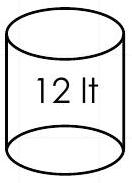
\includegraphics[max width=\textwidth, alt={}, center]{6dac6155-c874-45cc-9ccc-317741928334-113_183_132_495_1679}\\
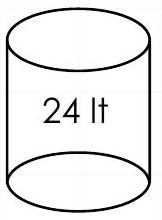
\includegraphics[max width=\textwidth, alt={}, center]{6dac6155-c874-45cc-9ccc-317741928334-113_220_162_458_1858}\\
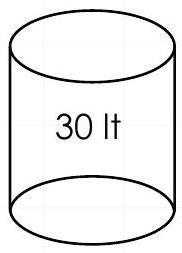
\includegraphics[max width=\textwidth, alt={}, center]{6dac6155-c874-45cc-9ccc-317741928334-113_253_182_425_2058}
  \item Si a es un número par y b es un número impar, ¿cuál de las siguientes expresiones representa un número par?\\
A) $a+b$\\
B) $2 a-b$\\
C) $3 a+3 b$\\
D) $5 a+4 b$
  \item Dos luces intermitentes se encienden con intervalos de 42 y 54 segundos, respectivamente. Si a las 10 horas y 15 minutos se encuentran ambas encendidas, ¿a qué hora estarán nuevamente ambas encendidas simultáneamente?\\
A) $10 \mathrm{hr} \cdot 21 \mathrm{~min} \cdot 18 \mathrm{seg}$\\
B) $10 \mathrm{hr} \cdot 21 \mathrm{~min} \cdot 36 \mathrm{seg}$\\
C) $10 \mathrm{hr} \cdot 21 \mathrm{~min} \cdot 42 \mathrm{seg}$\\
D) $10 \mathrm{hr} \cdot 15 \mathrm{~min} \cdot 54 \mathrm{seg}$
  \item Una habitación se encuentra a $7^{\circ} \mathrm{C}$. Si con determinada estufa, la temperatura asciende $2^{\circ} \mathrm{C}$ cada 10 minutos, ¿al cabo de cuánto tiempo la temperatura de la habitación será de $21^{\circ} \mathrm{C}$ ?\\
A) 14 minutos.\\
B) 35 minutos.\\
C) 1 hora y 10 minutos.\\
D) 2 horas y 20 minutos.
  \item Victoria tiene $\$ 38.000$ en efectivo, gasta $\$ 4.500$ en una entrada al cine, luego saca de su cuenta bancaria $\$ 20.000$ y compra un regalo a su mamá por un valor de $\$ 12.000$. ¿Cuál de las siguientes expresiones permite calcular el dinero en efectivo que le queda a Victoria?\\
A) $38.000-4.500+20.000$\\
B) $38.000-4.500-20.000-12.000$\\
C) $38.000-4.500+20.000+12.000$\\
D) $38.000-4.500+20.000-12.000$
\end{enumerate}

\section*{Z Preuniversitario Zenit}
\section*{EJERCICIOS M2}
\begin{enumerate}
  \item Sean $a>b$ y $b>c$, siendo $a$, b y $c$ números enteros. Si $b=0$, ¿cuál de las siguientes relaciones es verdadera?\\
A) $a \cdot c>0$\\
B) $a \cdot b>b$\\
C) $c^{2}<0$\\
D) $a-c>0$
  \item Se puede determinar que el número entero p es par si:\\
(1) El doble de p es par.\\
(2) El quíntuple de p es par.\\
A) (1) por sí sola.\\
B) (2) por sí sola.\\
C) Ambas juntas, (1) y (2).\\
D) Cada una por sí sola, (1) o (2).\\
E) Se requiere información adicional.
  \item Si A, B, C y D son números enteros tales que A $>B, C>D, B<D$ y C $<A$. El orden decreciente de ellos es:\\
A) $B D C A$\\
B) $A C D B$\\
C) $A C B D$\\
D) BDAC
  \item En una competencia de ciclismo, un corredor gana A carreras y pierde B carreras. Para determinar su puntaje final de la competencia, a las carreras ganadas se le restan el triple de las carreras perdidas. ¿Cuál es su puntaje final en la competencia?\\
A) $3 A-3 B$\\
B) $3 \mathrm{~A}-\mathrm{B}$\\
C) $A-3 B$\\
D) $A-\frac{1}{3} B$
  \item Si $A^{*}=A^{2}+1$, entonces $\left(3^{*}+1\right)^{*}=$\\
A) 49\\
B) 50\\
C) 100\\
D) 121\\
E) 122
  \item Si $a$ y $b$ son enteros y la suma de $a \cdot b$ y $b$ es impar, ¿cuál de las siguientes aseveraciones es verdadera?\\
A) $a$ y $b$ son ambos pares.\\
B) $a$ y $b$ son ambos impares.\\
C) $a$ es par y $b$ es impar.\\
D) $a$ es impar y $b$ es par.
  \item Sea $n$ un número entero. La expresión $3 \cdot(3+n)$ representa un múltiplo de 6 si:\\
(1) n es un número impar.\\
(2) $n+1$ es un número par.\\
A) (1) por sí sola.\\
B) (2) por sí sola.\\
C) Ambas juntas, (1) y (2).\\
D) Cada una por sí sola, (1) o (2).\\
E) Se requiere información adicional.
  \item ¿Qué valor toma la expresión $-b^{2} \cdot a^{-3}$, cuando $a=-3, b=-2$ ?\\
A) $\frac{9}{8}$\\
B) $-\frac{7}{9}$\\
C) $\frac{4}{27}$\\
D) $-\frac{4}{27}$\\
E) Ninguna de las anteriores
  \item ¿Cuál de las siguientes afirmaciones es verdadera?\\
A) El 1 es un número compuesto.\\
B) Todo número entero elevado a cero es 1.\\
C) El 1 es múltiplo de todos los números enteros.\\
D) El 1 es divisor de todos los números naturales.\\
E) El 1 es el neutro aditivo en los enteros.
  \item Sean los números enteros $a$, b y c. Se puede determinar cuál de ellos es el menor si:\\
(1) $a-b<0$\\
(2) $a-c>0$\\
A) (1) por sí sola.\\
B) (2) por sí sola.\\
C) Ambas juntas, (1) y (2).\\
D) Cada una por sí sola, (1) o (2).\\
E) Se requiere información adicional.
  \item Si el sucesor de un número es $\mathrm{m}+3$, entonces el doble del antecesor del número es:\\
A) $m+1$\\
B) $m+2$\\
C) $2 m+1$\\
D) $2 m+2$
  \item Si $m$ y $n$ son dos enteros consecutivos tales que $m<n$, entonces $n-m$ es:\\
A) 0\\
B) 1\\
C) $m^{2}+m$\\
D) $2 m+1$
  \item ¿Cuál es la cifra de la unidad de la operatoria $2^{42}+3^{901}$ ?\\
A) 2\\
B) 5\\
C) 7\\
D) 9
  \item Si N es un número entero, ¿cuál de las siguientes afirmaciones es verdadera?\\
A) ( $N^{2}-1$ ) es el entero antecesor del cuadrado de $N$.\\
B) - $(\mathrm{N}-1)$ es el entero antecesor de N .\\
C) $(N+1)^{2}$ es el entero sucesor del cuadrado de $N$.\\
D) $2 \mathrm{~N}-2$ es el entero antecesor del doble de N .
  \item Se puede asegurar que $P$ es un número divisible por 8 si:\\
(1) Sus últimas cuatro cifras son ceros.\\
(2) Su última cifra es número par.\\
A) (1) por sí sola.\\
B) (2) por sí sola.\\
C) Ambas juntas, (1) y (2).\\
D) Cada una por sí sola, (1) o (2).\\
E) Se requiere información adicional.
  \item Sean $a, b, c$ y d cuatro números primos distintos. El recíproco del cociente entre el máximo común divisor y el mínimo común múltiplo entre ellos es:\\
A) $a b c d$\\
B) $\frac{1}{a b c d}$\\
C) $\frac{a b c d}{4}$\\
D) $4 a b c d$
  \item Una persona debe reunir $A$ pesos. Primero reúne $B$ pesos y luego gasta $C$ pesos. ¿Cuánto le falta, en pesos, para completar el monto que necesita, si $\mathrm{A}>\mathrm{B}>\mathrm{C}$ ?\\
A) $A+B-C$\\
B) $C+A-B$\\
C) $-A-(C-B)$\\
D) $A-(B+C)$
  \item Benjamín tiene ahorrado 12 monedas de $\$ 50 ; 25$ monedas de $\$ 100$ y el resto en monedas de $\$ 500$, de manera que en total tiene $\$ 7.100$. Si cambia todas las monedas de $\$ 500$, por monedas de $\$ 50$, ¿cuántas monedas tendrá en total?\\
A) 8\\
B) 80\\
C) 105\\
D) 117
  \item Los números siguientes ordenados de manera creciente son:
\end{enumerate}

$$
A=20^{10}, B=3^{40}, C=12^{20}, D=2^{50}
$$

A) $A, D, B, C$\\
B) $A, B, D, C$\\
C) $D, B, C, A$\\
D) $D, B, A, C$\\
E) $C, B, D, A$\\
20. Ana tiene $X$ cantidad de dinero en efectivo, gasta $A$ en un almuerzo, luego retira de su cuenta bancaria $B$ y compra un libro por C. ¿Cuál de las siguientes expresiones permite calcular el dinero en efectivo que le queda a Ana?\\
A) $X-A+B-C$\\
B) $X-A-B-C$\\
C) $X+A-B+C$\\
D) $X+A+B+C$

\section*{CAPÍTULO 1 \\
 RESPUESTAS}
\begin{center}
\begin{tabular}{|l|l|l|l|l|l|l|l|l|l|l|l|}
\hline
1. B &  & 1. & A & 21. & A & 41. & C & 61. & C & 1. & D \\
\hline
2. & B & 2. & B & 22. & C & 42. & C & 62. & D & 2. & B \\
\hline
3. & B & 3. & A & 23. & C & 43. & C & 63. & A & 3. & B \\
\hline
4. & A & 4. & C & 24. & D & 44. & A & 64. & C & 4. & C \\
\hline
5. & A & 5. & B & 25. & C & 45. & D & 65. & D & 5. & E \\
\hline
6. & B & 6. & D & 26. & A & 46. & C &  &  & 6. & C \\
\hline
7. & B & 7. & C & 27. & D & 47. & A &  &  & 7. & D \\
\hline
8. & C & 8. & C & 28. & A & 48. & C &  &  & 8. & C \\
\hline
9. & A & 9. & D & 29. & D & 49. & C &  &  & 9. & D \\
\hline
10. & C & 10. & C & 30. & B & 50. & C &  &  & 10. & C \\
\hline
11. & B & 11. & C & 31. & D & 51. & C &  &  & 11. & D \\
\hline
12. & C & 12. & D & 32. & B & 52. & B &  &  & 12. & B \\
\hline
13. & A & 13. & A & 33. & B & 53. & A &  &  & 13. & C \\
\hline
14. & D & 14. & D & 34. & B & 54. & B &  &  & 14. & A \\
\hline
15. & D & 15. & C & 35. & A & 55. & C &  &  & 15. & A \\
\hline
16. & C & 16. & B & 36. & C & 56. & C &  &  & 16. & A \\
\hline
17. & B & 17. & B & 37. & B & 57. & C &  &  & 17. & B \\
\hline
18. & C & 18. & C & 38. & C & 58. & A &  &  & 18. & D \\
\hline
19. & B & 19. & D & 39. & D & 59. & C &  &  & 19. & A \\
\hline
20. & C & 20. & B & 40. & D & 60. & A &  &  & 20. & A \\
\hline
\end{tabular}
\end{center}


\end{document}